A CREUSER :

	à cahque coup on va chercher à augmenter ou diminuer siuvant lsens de parcrousrs 

	par contre aux extrémités, on s'autoirsent à fair une boucle !



Il se trouve que la méthode \quote{on avance au mieux} n'est pas la plus efficace comme le montre l'exemple suivant où six mouvements totalement inutiles sont effectués si bien que l'on n'a toujours pas gagné à la neuvième étape.

\vspace{-0.4em}
\begin{multicols}{2}
	\begin{center}   % [4, 4, None, 0, 1, 1, 2, 2, 3, 3]
		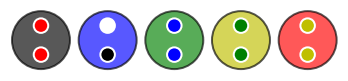
\includegraphics[scale= 0.45]{content/optimal/wheredowego/algo_bubble/000.png}

		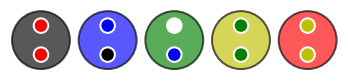
\includegraphics[scale= 0.45]{content/optimal/wheredowego/algo_bubble/001.png}

		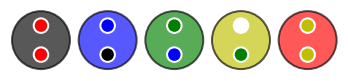
\includegraphics[scale= 0.45]{content/optimal/wheredowego/algo_bubble/002.png}

		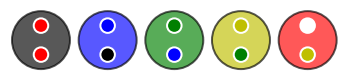
\includegraphics[scale= 0.45]{content/optimal/wheredowego/algo_bubble/003.png}

		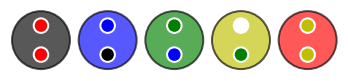
\includegraphics[scale= 0.45]{content/optimal/wheredowego/algo_bubble/004.png}
	\end{center}

	\columnbreak
	\begin{center}   % [4, 4, None, 0, 1, 1, 2, 2, 3, 3]
		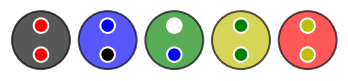
\includegraphics[scale= 0.45]{content/optimal/wheredowego/algo_bubble/005.png}

		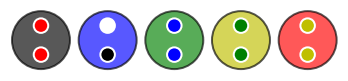
\includegraphics[scale= 0.45]{content/optimal/wheredowego/algo_bubble/006.png}

		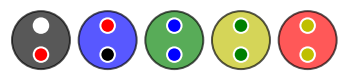
\includegraphics[scale= 0.45]{content/optimal/wheredowego/algo_bubble/007.png}

		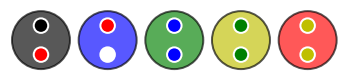
\includegraphics[scale= 0.45]{content/optimal/wheredowego/algo_bubble/008.png}

		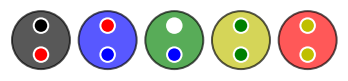
\includegraphics[scale= 0.45]{content/optimal/wheredowego/algo_bubble/009.png}
	\end{center}
\end{multicols}


\medskip

Or on peut gagner ici en seulement 9 coups ! Voici les mouvements à faire
\footnote{
	Notez au passage les enseignements que l'on peut tirer d'une configuration très, très particulière.
}.   DESSIN FAUX !!!!!!!!!!!!!

\vspace{-0.4em}
\begin{multicols}{2}
	\begin{center}   % [4, 4, None, 0, 1, 1, 2, 2, 3, 3]
		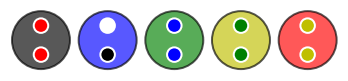
\includegraphics[scale= 0.45]{content/optimal/wheredowego/algo_bubble/000.png}

		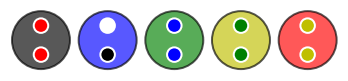
\includegraphics[scale= 0.45]{content/optimal/wheredowego/algo_bubble/000.png}

		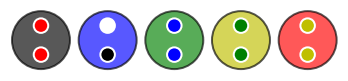
\includegraphics[scale= 0.45]{content/optimal/wheredowego/algo_bubble/000.png}

		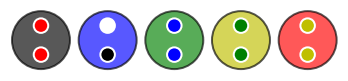
\includegraphics[scale= 0.45]{content/optimal/wheredowego/algo_bubble/000.png}

		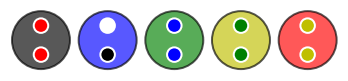
\includegraphics[scale= 0.45]{content/optimal/wheredowego/algo_bubble/000.png}
	\end{center}

	\columnbreak
	\begin{center}   % [4, 4, None, 0, 1, 1, 2, 2, 3, 3]
		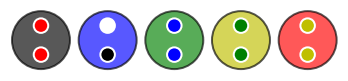
\includegraphics[scale= 0.45]{content/optimal/wheredowego/algo_bubble/000.png}

		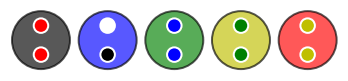
\includegraphics[scale= 0.45]{content/optimal/wheredowego/algo_bubble/000.png}

		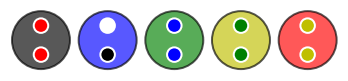
\includegraphics[scale= 0.45]{content/optimal/wheredowego/algo_bubble/000.png}

		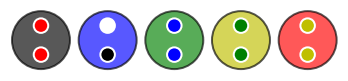
\includegraphics[scale= 0.45]{content/optimal/wheredowego/algo_bubble/000.png}

		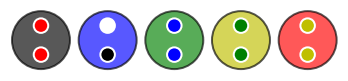
\includegraphics[scale= 0.45]{content/optimal/wheredowego/algo_bubble/000.png}
	\end{center}
\end{multicols}


\medskip

Commençons par proposer une nouvelle modélisation du jeu qui soit bien plus fine que celles utilisées dans les deux sections précédentes. 
Que cherche-t-on à faire ? Trouver une solution peu coûteuse. Très bien ! Mais dans ce cas, comment évalue-t-on ce coup ? Nous choisissons de chercher à minimiser le nombre de déplacements du trou (donc toute opération autre que le déplacement d'un jeton ne sera pas comptabilisée).
Dans le premier cas ci-dessus, le coût est strictement plus grand que $9$, tandis que dans le second cas, il vaut exactement $9$. 


\medskip

Soit une configuration $\cal C$

??????????????????????????????????????????
notation en ligne car pratique mais ici on s'autorise le passage de la base tout à droite à celle tout à gauche
??????????????????????????????????????????

. Pour chaque jeton $j$, nous notons $deg \ j$ son degré d'éloignement qui est égal par définition aux nombres de bases entre sa base comprise et la base de sa couleur.
Par exemple, au début des exemples ci-dessus, tous les jetons ont un degré d'éloignement égal à un.


\medskip

Nous pouvons alors proposer la troisième méthode suivante (notez la concision de l'algorithme).   PAS BON PAS BON PAS BON PAS BON PAS BON PAS BON PAS BON PAS BON PAS BON PAS BON ( voir juste parès !!!!

\bigskip

\begin{algo}
	\Data{une configuration quelconque de début de jeu}
	\Result{une configuration où tous les jetons sont rentrées dans leur base}
	\vspace{0.4em}
    \Begin{
		\vspace{0.4em}
		\While{la configuration contient un jeton qui n'est pas dans sa base}{
			\vspace{0.4em}
			$j_1$ , $j_2$ , $j_3$ et $j_4$ désignent les jetons déplaçables.
			\\
			\vspace{0.4em}
			Pour $k$ allant de $1$ à $4$, on note $d_k$ est le dégré d'éloignement du jeton $j_k$ s'il était déplacé.
			\\
			\vspace{0.4em}
			Déplacer réellement un jeton $j_k$, éventuellement choisi au hasard, tel que $d_k$ soit minimal.
		}
    }
\end{algo}


\bigskip

Les instructions étant sans ambiguïté, nous allons pouvoir nous attaquer très sérieusement à la validation des propriétés de \quote{finitude} et de \quote{résolution}.

\begin{proof}
	????????????????????
	
	CODER POUR VOIR SI CEL MARCHE 
	
	PAR EXEMPLe, faire gaffe au cas ou les quatre jetons déplaçables ont le même degré dans la config du moment
	
	r r t n j j b b v v
	
	r r j n t j b b v v
	
	pas possible car boucle infinie possible
\end{proof}
